\begin{frame}
    \frametitle{The Five Color Theorem}
    \begin{theorem}<1->
        Every planar graph can be colored in at most five colors.
    \end{theorem}
    \begin{proof}<2->
            Every planar graph $G$ has a vertex of $\deg(v)\leq 5$.
            \begin{itemize}
                \item If $\deg(v) \leq 4$, can use fifth color.
                \item If $\deg(v) = 5$, can always free up a color.
            \end{itemize}
            Remove $v$ from the graph and repeat until there are no vertices left. Add back and color these vertices until we obtain a coloring of $G$.
    \end{proof}
\end{frame}

\begin{frame}
    \frametitle{The Five Color Theorem}
    \begin{alertblock}{Most important argument}
        If $\deg(v)=5$, can always free up a color.
    \end{alertblock}
    \vspace{0.5cm}
    \begin{minipage}{0.59\textwidth}
        \begin{itemize}
            \item If there is an $ac$-chain, then we have isolated $b$. Therefore, there can not be a $bd$-chain from $b$ to $d$. We may flip the $bd$-chain of $b$ to free up the color $d$. 
            \item If there is no $ac$-chain, then $a$ and $c$ are not connected. So we may flip the $ac$-chain of $a$ to free up the color $c$.
        \end{itemize}
    \end{minipage}
    \begin{minipage}{0.39\textwidth}
        \centering
        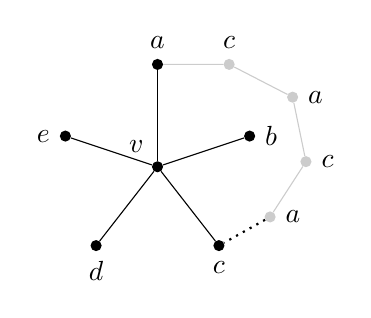
\begin{tikzpicture}[scale=1.3]
            \node[circle, fill, scale=0.015cm, label=above left:$v$] (c) at (0, 0) {};
            \node[circle, fill, scale=0.015cm, label=above:$a$] (l1) at (0, 1) { };
            \node[circle, fill, scale=0.015cm, label=right:$b$] (l2) at (0.9, 0.30) { };
            \node[circle, fill, scale=0.015cm, label=below:$c$] (l3) at (0.6, -0.77) {};
            \node[circle, fill, scale=0.015cm, label=below:$d$] (l4) at (-0.6, -0.77) {};
            \node[circle, fill, scale=0.015cm, label=left:$e$] (l5) at (-0.9, 0.30) {};
            \node[circle, fill, scale=0.015cm, label=above:$c$, opacity=0.2] (c1) at (0.7, 1) {};
            \node[circle, fill, scale=0.015cm, label=right:$a$, opacity=0.2] (c2) at (1.32, 0.68) {};
            \node[circle, fill, scale=0.015cm, label=right:$c$, opacity=0.2] (c3) at (1.45, 0.05) {};
            \node[circle, fill, scale=0.015cm, label=right:$a$, opacity=0.2] (c4) at (1.1, -0.49) {};
    
            \draw (c) -- (l1);
            \draw (c) -- (l2);
            \draw (c) -- (l3);
            \draw (c) -- (l4);
            \draw (c) -- (l5);
    
            \draw[opacity=0.2] (l1) -- (c1) -- (c2) -- (c3) -- (c4);
            \draw[dotted, thick] (c4) -- (l3);
            
        \end{tikzpicture}
    \end{minipage}
\end{frame}